\section*{Appendix}

We show full quantitative details in Appendix \ref{sec:quant}. We also discuss training details in Appendix \ref{sec:train}. Finally, we show results on the TID2013 dataset~\cite{ponomarenko2015image} in Appendix \ref{sec:tid}.

\section{Quantitative Results}
\label{sec:quant}

\begin{figure*}[t]
\centering
\begin{tabular}{*{2}{c@{\hspace{3px}}}}
\textbf{Distortions (Traditional)} & \textbf{Distortions (CNN-Based)} \\
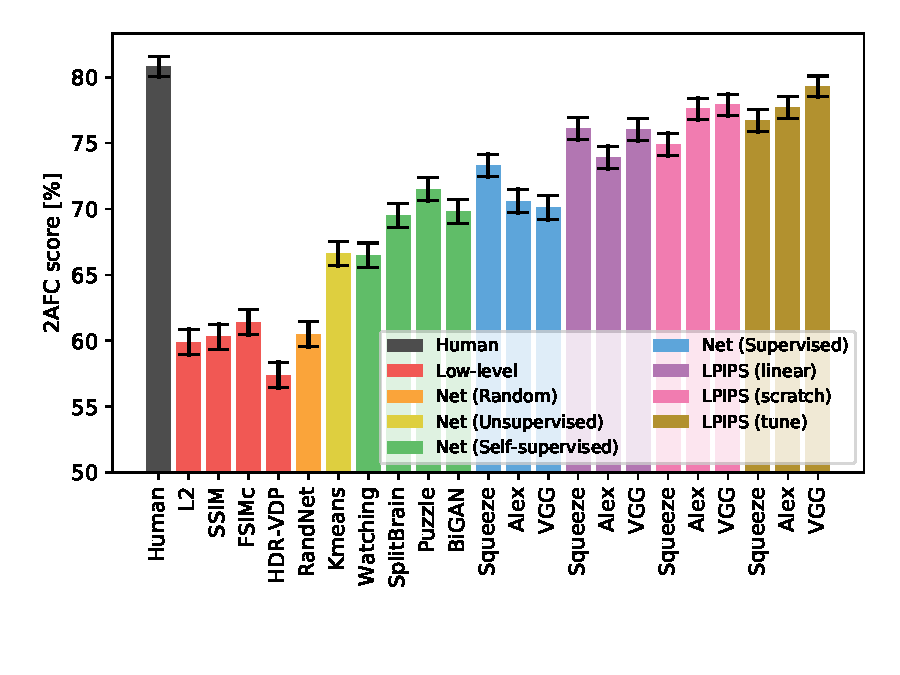
\includegraphics[width=.5\linewidth]{imgs/3_traditional.pdf}
&
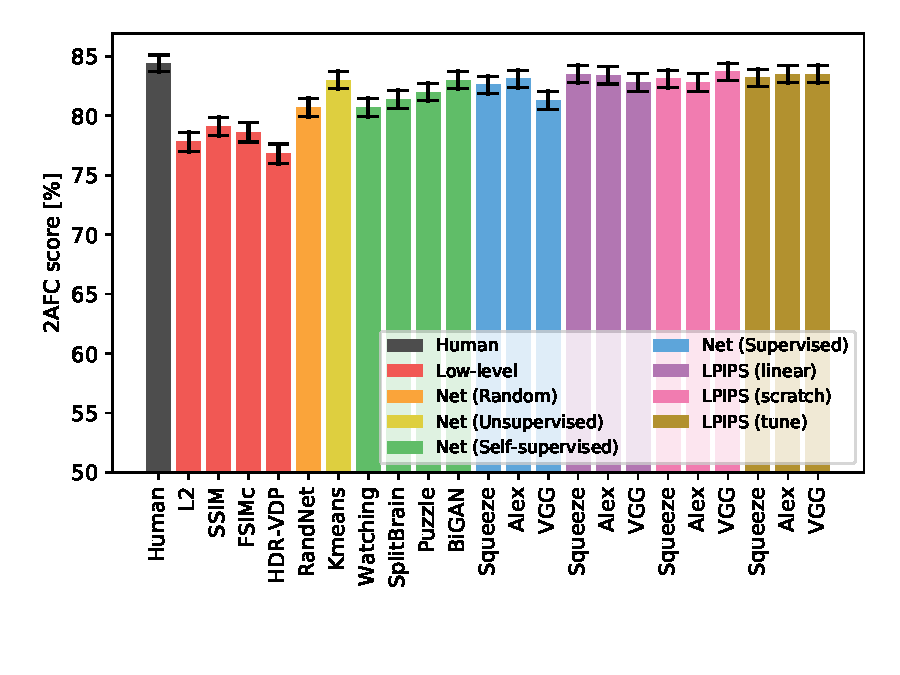
\includegraphics[width=.5\linewidth]{imgs/4_cnn-based.pdf} \\
\end{tabular}
\vspace{-10mm}
\caption{\textbf{Individual results} (left) traditional distortions (right) CNN-based distortions}
\label{fig:quant1}
\end{figure*}

\begin{figure*}[t]
\centering
\begin{tabular}{*{2}{c@{\hspace{3px}}}}
\textbf{Real Algorithms (Superresolution)} & \textbf{Real Algorithms (Frame Interpolation)} \\
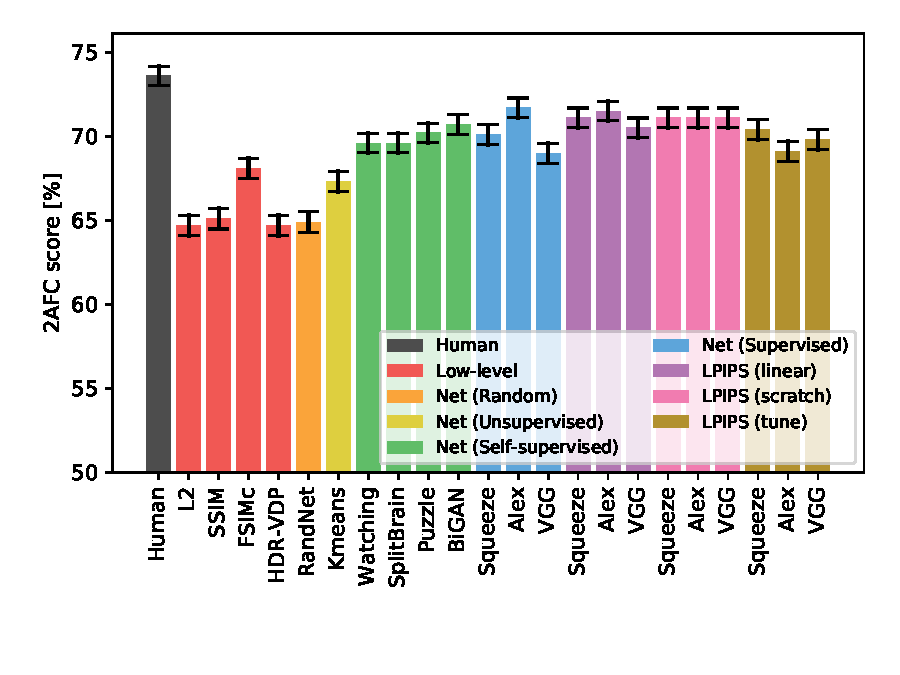
\includegraphics[width=.5\linewidth]{imgs/5_superres.pdf} &
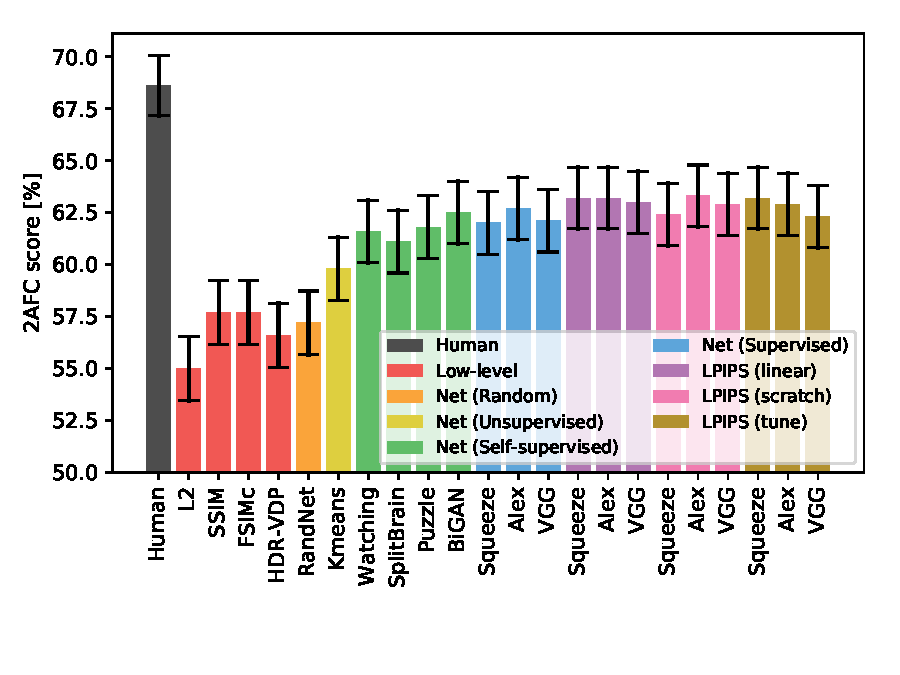
\includegraphics[width=.5\linewidth]{imgs/8_frame_interp.pdf} \\
\end{tabular}
\vspace{-10mm}
\caption{\textbf{Individual results} (left) superresolution (right) frame interpolation}
\label{fig:quant2}
\end{figure*}

\begin{figure*}[h!]
\centering
\begin{tabular}{*{2}{c@{\hspace{3px}}}}
\textbf{Real Algorithms (Video Deblurring)} & \textbf{Real Algorithms (Colorization)} \\
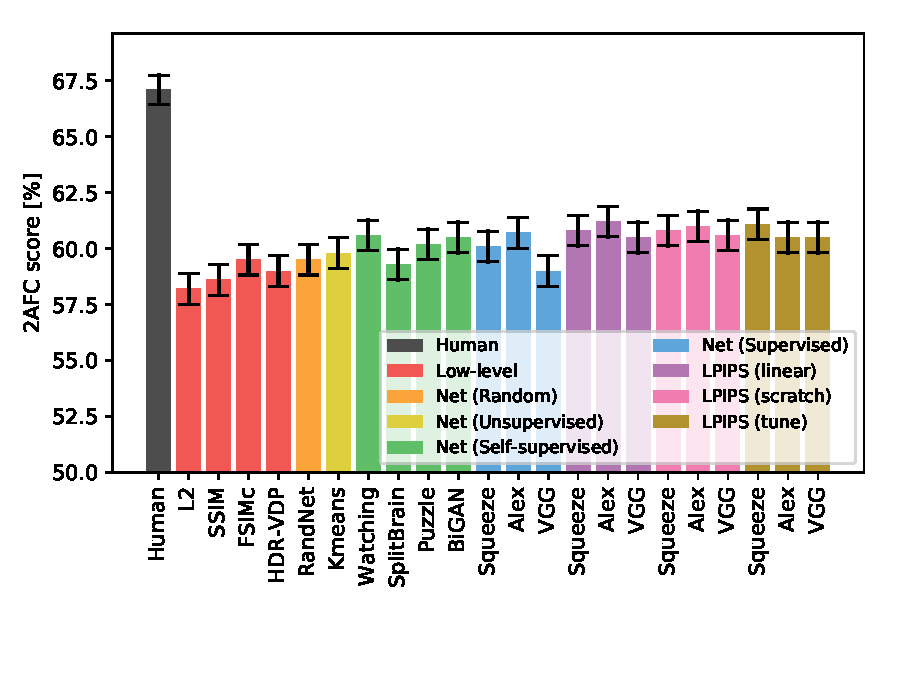
\includegraphics[width=.5\linewidth]{imgs/6_deblur.pdf} &
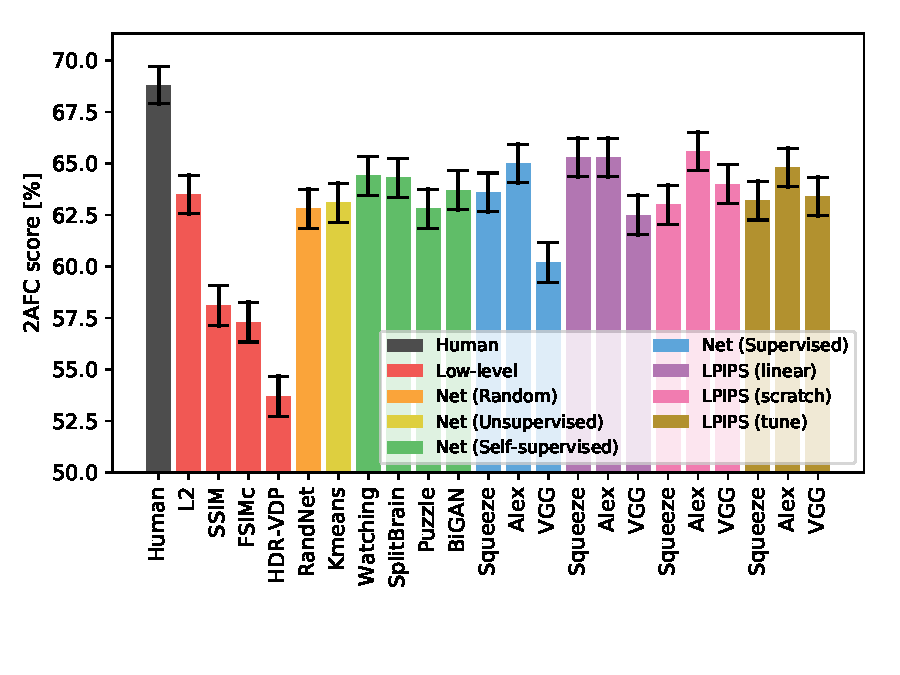
\includegraphics[width=.5\linewidth]{imgs/7_color.pdf} \\
\end{tabular}
\vspace{-10mm}
\caption{\textbf{Individual results} (left) video deblurring (right) colorization}
\label{fig:quant3}
\end{figure*}

\subfile{tables/results}


\begin{figure*}
\centering
\begin{subfigure}{1.\textwidth}
  \centering
  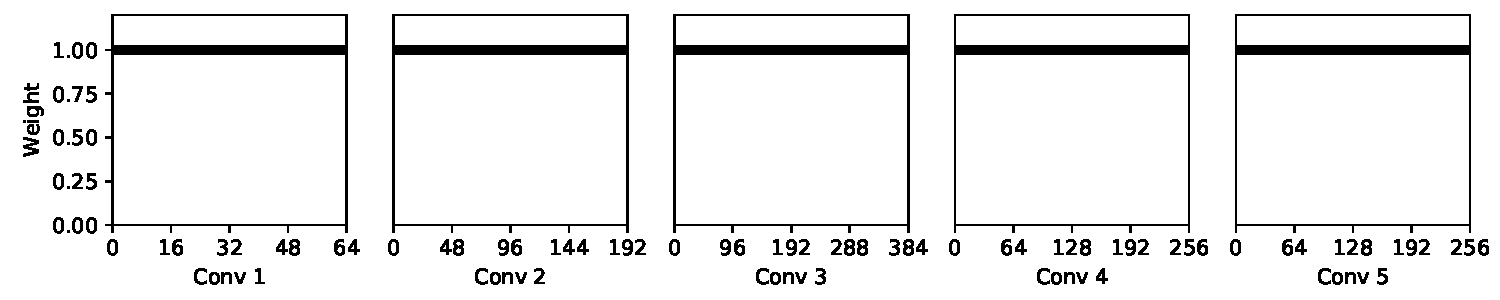
\includegraphics[width=1.\linewidth]{imgs/weights_subplotted_alex_ones.pdf}
  \vspace{-6mm}
  \caption{\textbf{Unlearned weights for AlexNet model (cosine distance)}}
  \label{fig:weights_ones}
\end{subfigure}

\begin{subfigure}{1.\textwidth}
  \centering
    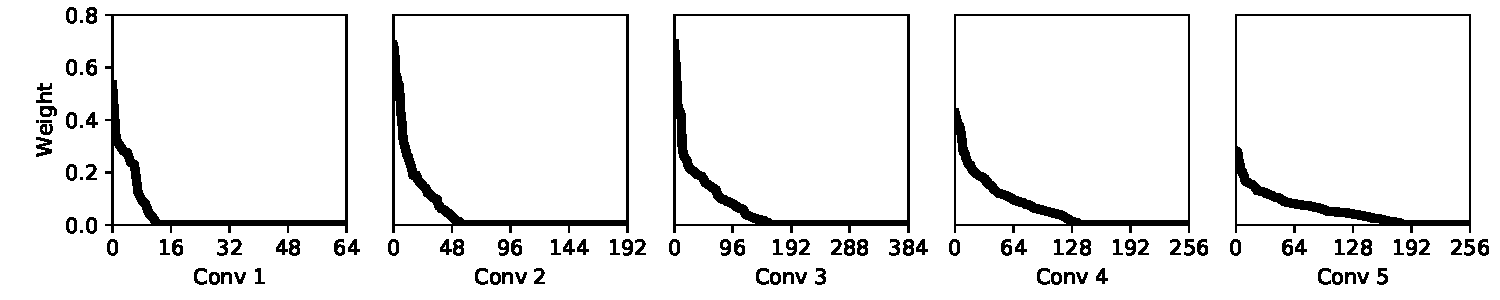
\includegraphics[width=1.\linewidth]{imgs/weights_subplotted_alex.pdf}
    \vspace{-6mm}
    \caption{\textbf{Learned weights from \textit{Alex--lin} model}}
\label{fig:weights_learned}
\end{subfigure}

\begin{subfigure}{1.\textwidth}
  \centering
    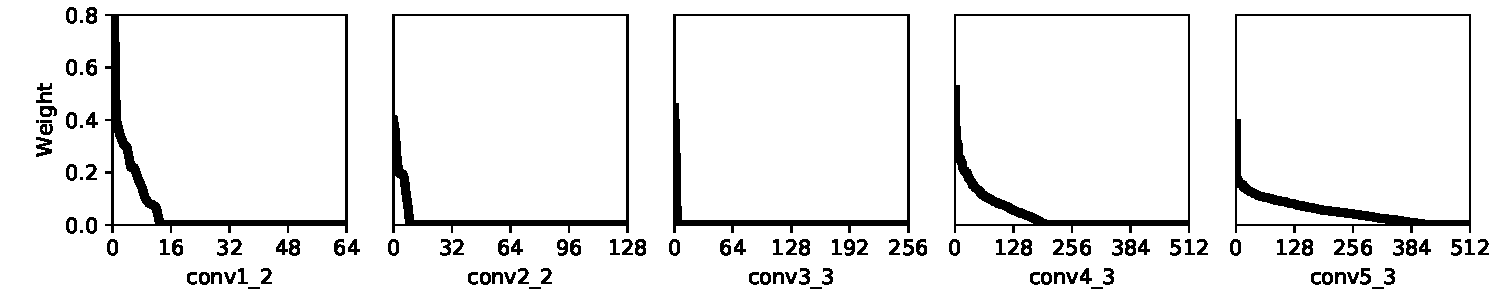
\includegraphics[width=1.\linewidth]{imgs/weights_subplotted_vgg.pdf}
    \vspace{-6mm}
    \caption{\textbf{Learned weights from \textit{VGG--lin} model}}
\label{fig:weights_learned_vgg}
\end{subfigure}

\begin{subfigure}{1.\textwidth}
  \centering
    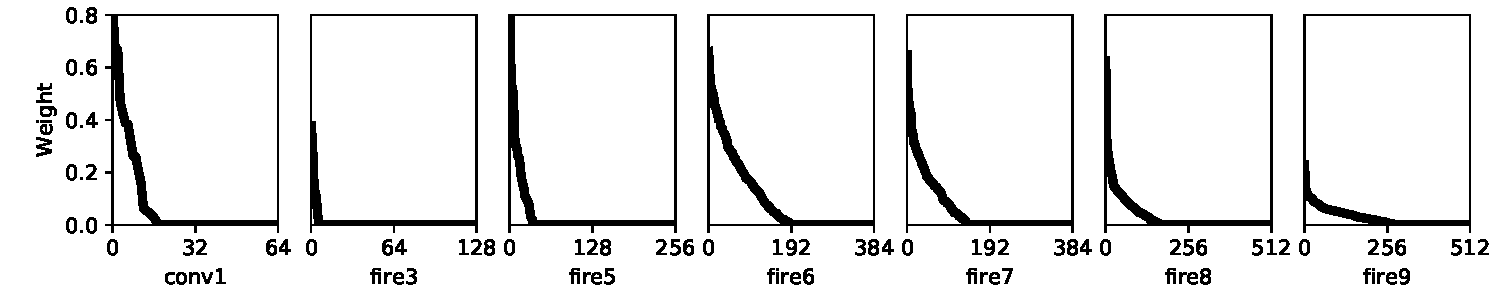
\includegraphics[width=1.\linewidth]{imgs/weights_subplotted_squeeze.pdf}
    \vspace{-6mm}
    \caption{\textbf{Learned weights from \textit{Squeeze--lin} model}}
\label{fig:weights_learned_squeeze}
\end{subfigure}

\vspace{-2mm}
\caption{\textbf{Learned linear weights by layer.} (a) Unlearned weights correspond to using weighting 1 for each channel in each layer, which results in computing cosine distance. (b) We show the learned weights from each layer of our \textit{Alex--lin} model. This is the $w$ term in Figure~\ref{fig:network}. Each subplot shows the channel weights from each layer, sorted in descending order. The x-axis shows the channel number, and y-axis shows the weight. Weights are restricted to be non-negative, as image patches should not have negative distance. (c,d) Same as (b), but with the \textit{VGG--lin} and \textit{Squeeze--lin} models.}
\label{fig:weights}
\vspace{-4mm}
\end{figure*}

\begin{figure*}
\centering
\begin{subfigure}{1.\textwidth}
  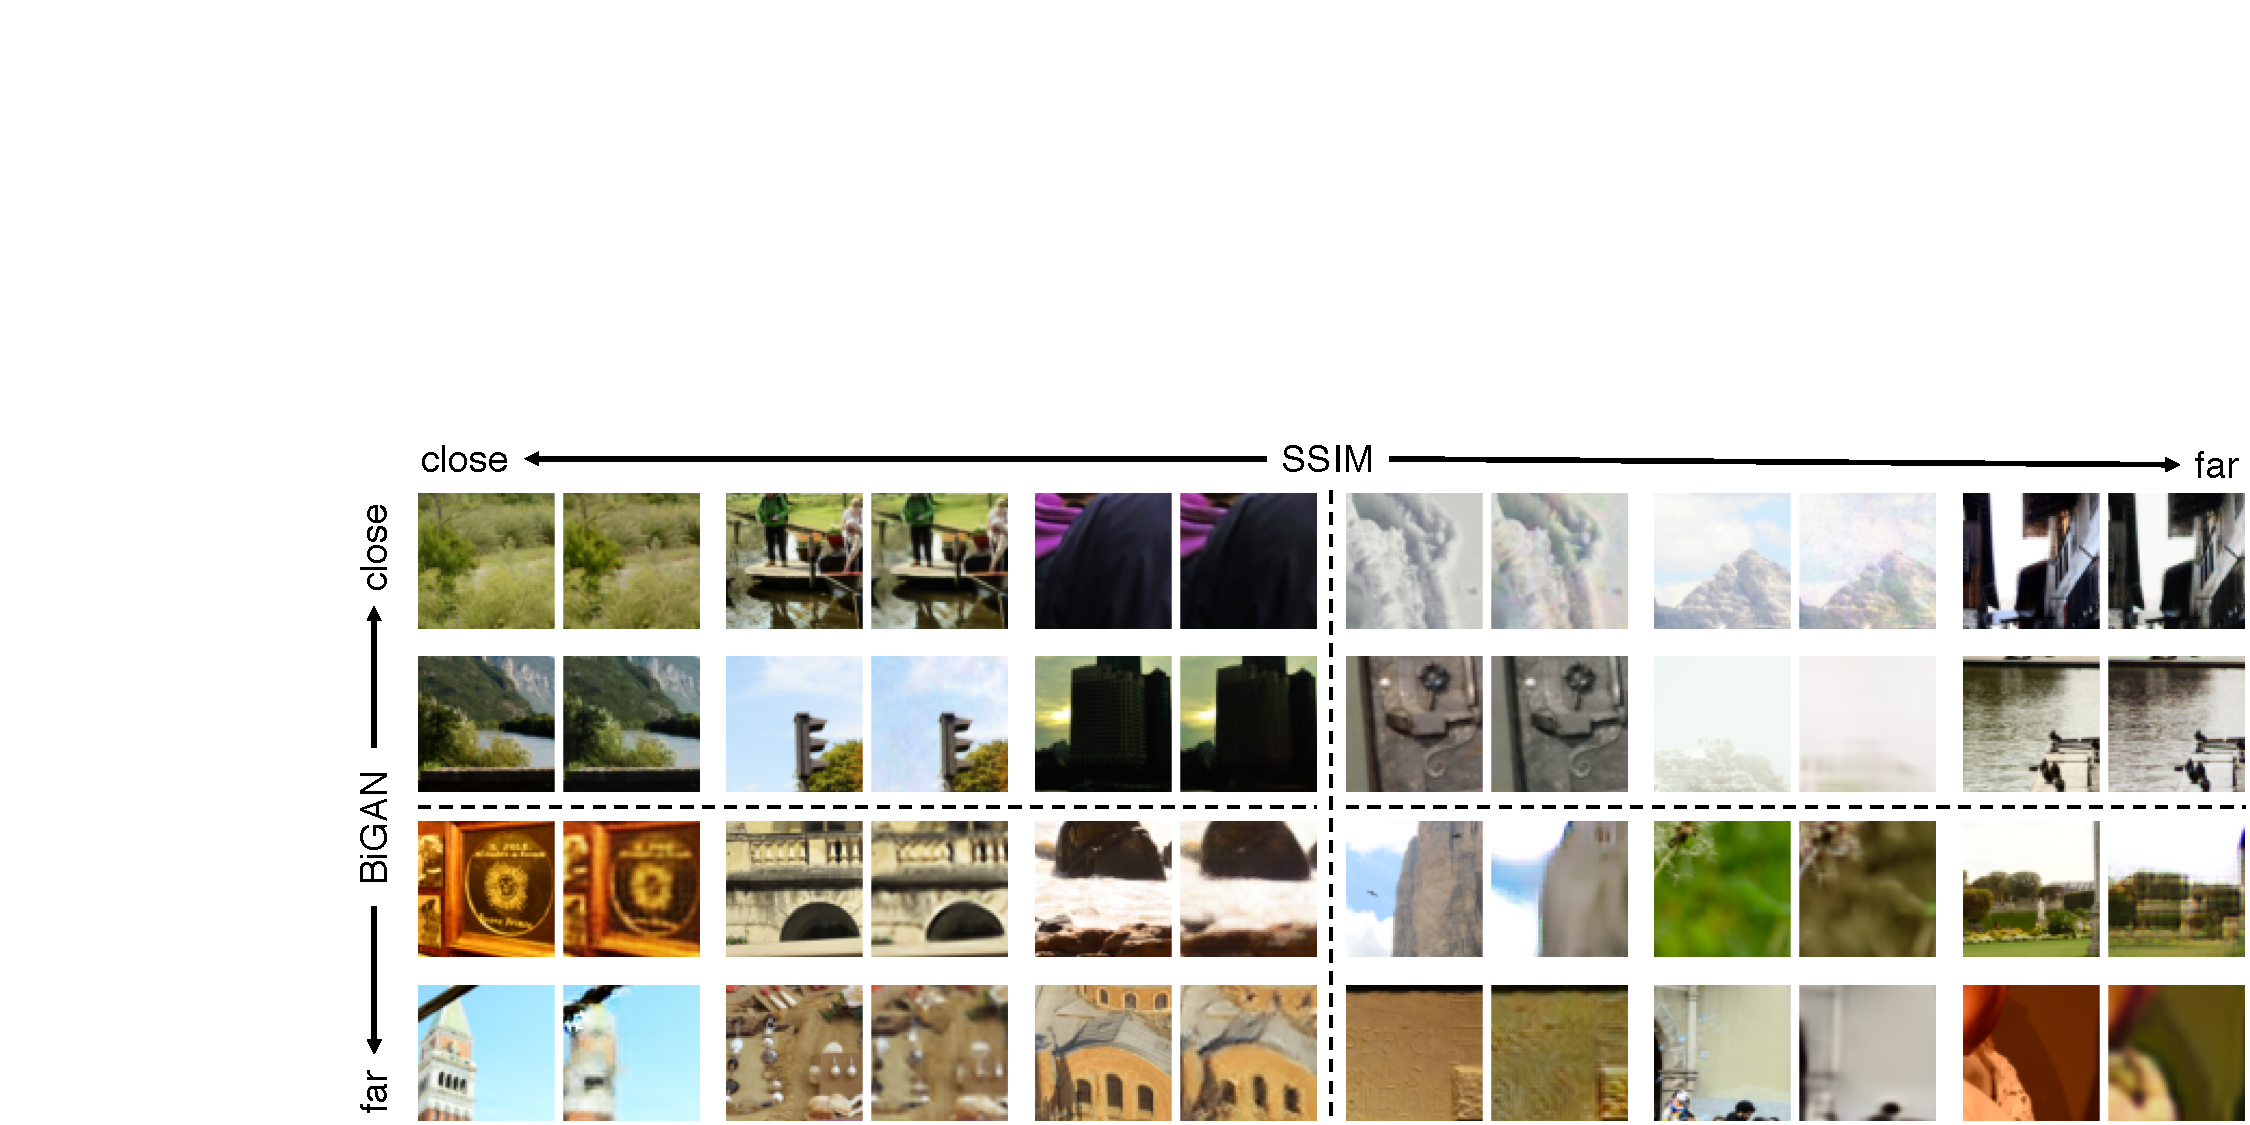
\includegraphics[width=1.\linewidth]{imgs/fig_comp_high.pdf}
\end{subfigure}
\vspace{-2mm}
\caption{\textbf{Qualitative comparisons on distortions.} We show qualitative comparison on CNN-based distortions, using the SSIM~\cite{wang2004image} metric and BiGAN network~\cite{donahue2016adversarial}. We show examples where both agree the patches are closer or far, and examples where the metrics disagree. A primary difference is that deep embeddings appear to be more sensitive to blur. Please see the appendix for additional examples.}
\label{fig:qual_comp}
\vspace{-4mm}
\end{figure*}

In Table~\ref{tab:res_quant}, we show full quantitative results across all validation sets and considered metrics, including low-level metrics, along with random, unsupervised, self-supervised, supervised, and perceptually-learned networks.

In Figures~\ref{fig:quant1}, ~\ref{fig:quant2}, ~\ref{fig:quant3}, we plot performance in individual validation sets. Figure~\ref{fig:quant1} shows our traditional and CNN-based distortions, and Figures~\ref{fig:quant2},~\ref{fig:quant3} show results on real algorithm applications individually.

\paragraph{Human performance} If humans chose patches \{$x_1$,$x_0$\} with fraction \{$p$,$1-p$\}, the theoretical maximum for an oracle is $\max(p,1-p)$. However, human performance is lower. If an agent chooses them with probability \{$q$,$1-q$\}, the agent will agree with $qp + (1-q)(1-p)$ humans on expectation. With a human agent, $q=p$, the expected human score is $p^2 + (1-p)^2$.

\paragraph{Linearly calibrating networks} Learning linear weights on top of the \tbfit{Alex} model achieves state-of-the-art results on the real algorithms test set. The \tbfit{linear} models have a learned linear layer on top of each channel, whereas the out-of-the-box versions weight each channel equally. In Figure~\ref{fig:weights_learned}, we show the learned weights for the \tbfit{Alex --frozen} model. The \texttt{conv1-5} layers contain 64, 192, 384, 256, and 256 channels, respectively, for a total of 1152 weights. For each layer, \texttt{conv1-5}, $79.7\%$, $71.4\%$, $56.8\%$, $46.5\%$, $27.7\%$, respectively, of the weights are zero. This means that a majority of the \texttt{conv1} and \texttt{conv2} units are ignored, and almost all of the \texttt{conv5} units are used. Overall, about half of the units are ignored. Taking the cosine distance is equivalent to setting all weights to 1 (Figure~\ref{fig:weights_ones}).

\paragraph{Data quantity for training models on distortions} The performance of the validation set on our distortions ($80.6\%$ and $81.4\%$ for \tbfit{Alex -- tune} and \tbfit{VGG -- tune}, respectively), is almost equal to human performance of $82.6\%$. This indicates that our training set size of 150k patch pairs and 300k judgments is nearly large enough to fully explore the traditional and CNN-based distortions which we defined. However, there is a small gap between the \tbfit{tune} and \tbfit{scratch} models ($0.4\%$ and $0.6\%$ for \tbfit{Alex} and \tbfit{VGG}, respectively).

